On considère un cube $ABCDEFGH$ d'arête 8~cm et de centre $\Omega$.

\smallskip

Les points $P$, $Q$ et $R$ sont définis par $\vect{{AP}} = \dfrac{3}{4}\vect{{AB}}$ ; $\vect{{AQ}} = \dfrac{3}{4}\vect{{AE}}$ et $\vect{{FR}} = \dfrac{1}{4}\vect{{FG}}$.

\smallskip

On se place dans le repère orthonormé $\left({A};\vect{\imath},\vect{\jmath},\vect{k}\right)$ avec : $\vect{\imath} = \dfrac{1}{8}\vect{{AB}}$ ; $\vect{\jmath}= \dfrac{1}{8}\vect{{AD}}$ et $\vect{k} = \dfrac{1}{8}\vect{{AE}}$.

\begin{center}
	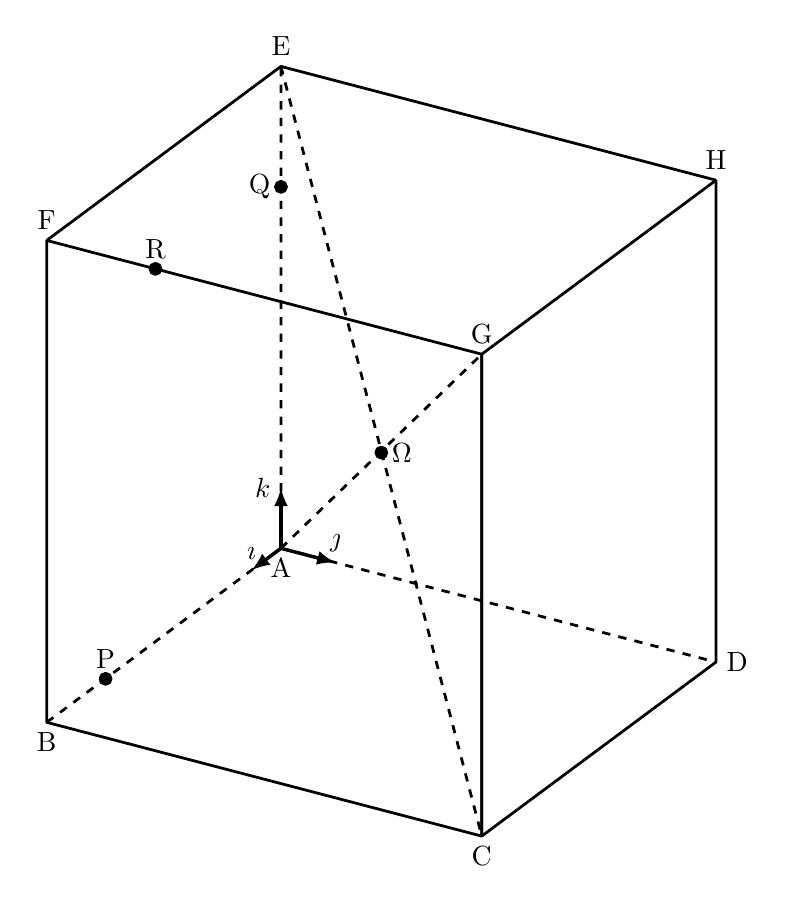
\begin{tikzpicture}[x=0.85cm,y=0.85cm,line width=1pt,line join=bevel,>=latex]
		%arêtes
		\draw (0,1.7)--(6.5,0)--(6.5,7.2)--(0,8.9)--cycle ; %BCGF
		\draw (6.5,0)--(10,2.6)--(10,9.8)--(6.5,7.2)--cycle ; %CDHG
		\draw (10,9.8)--(3.5,11.5)--(0,8.9) ; %HEF
		\draw[dashed] (0,1.7)--(3.5,4.3)--(3.5,11.5) ; %BAE
		\draw[dashed] (3.5,4.3)--(10,2.6) ; %AD
		\draw[dashed] (3.5,4.3)--(6.5,7.2) ; %AG
		\draw[dashed] (3.5,11.5)--(6.5,0) ; %EC
		%vecteurs
		\draw[->,line width=1.25pt] (3.5,4.3)--(3.0625,3.975) ;
		\draw[->,line width=1.25pt] (3.5,4.3)--(4.3125,4.0875) ;
		\draw[->,line width=1.25pt] (3.5,4.3)--(3.5,5.2) ;
		%labels simples
		\foreach \Point/\Nom/\Pos in {(0,1.7)/B/below,(6.5,0)/C/below,(6.5,7.2)/G/above,(0,8.9)/F/above,(10,2.6)/D/right,(10,9.8)/H/above,(3.5,11.5)/E/above,(3.5,4.3)/A/below}
		\draw \Point node[\Pos] {\Nom} ;
		%labels "dot"
		\foreach \Point/\Nom/\Pos in {(5,5.73)/$\Omega$/right,(0.88,2.35)/P/above,(3.5,9.7)/Q/left,(1.625,8.475)/R/above}
		\filldraw \Point circle[radius=2pt] node[\Pos] {\Nom} ;
		%labels vecteurs
		\foreach \Vecteur/\Nom/\Pos in {(3.0625,3.975)/$\vect{\imath}$/above,(4.3125,4.0875)/$\vect{\jmath}$/above,(3.5,5.2)/$\vect{k}$/left}
		\draw \Vecteur node[\Pos] {\Nom} ;
	\end{tikzpicture}
\end{center}

\textbf{Partie I}

\begin{enumerate}
	\item Dans ce repère, on admet que les coordonnées du point $R$ sont $(8;2;8)$. 
	
	Donner les coordonnées des points $P$ et $Q$.
	\item Montrer que le vecteur $\vect{n}(1;-5;1)$ est un vecteur normal au plan $(PQR)$.
	\item Justifier qu'une équation cartésienne du plan $(PQR)$ est $x - 5y + z - 6 = 0$.
\end{enumerate}

\textbf{Partie II}

\medskip

On note $L$ le projeté orthogonal du point $\Omega$ sur le plan $(PQR)$.

\begin{enumerate}
	\item Justifier que les coordonnées du point $\Omega$ sont $(4;4;4)$.
	\item Donner une représentation paramétrique de la droite $d$ perpendiculaire au plan $(PQR)$ et passant par $\Omega$.
	\item Montrer que les coordonnées du point $L$ sont $\left(\dfrac{14}{3}; \dfrac{2}{3};\dfrac{14}{3}\right)$
	\item Calculer la distance du point $\Omega$ au plan $(PQR)$.
\end{enumerate}

